\documentclass[border=10pt]{standalone}
\usepackage{tikz}
\usetikzlibrary{arrows.meta, shapes, calc}

\begin{document}

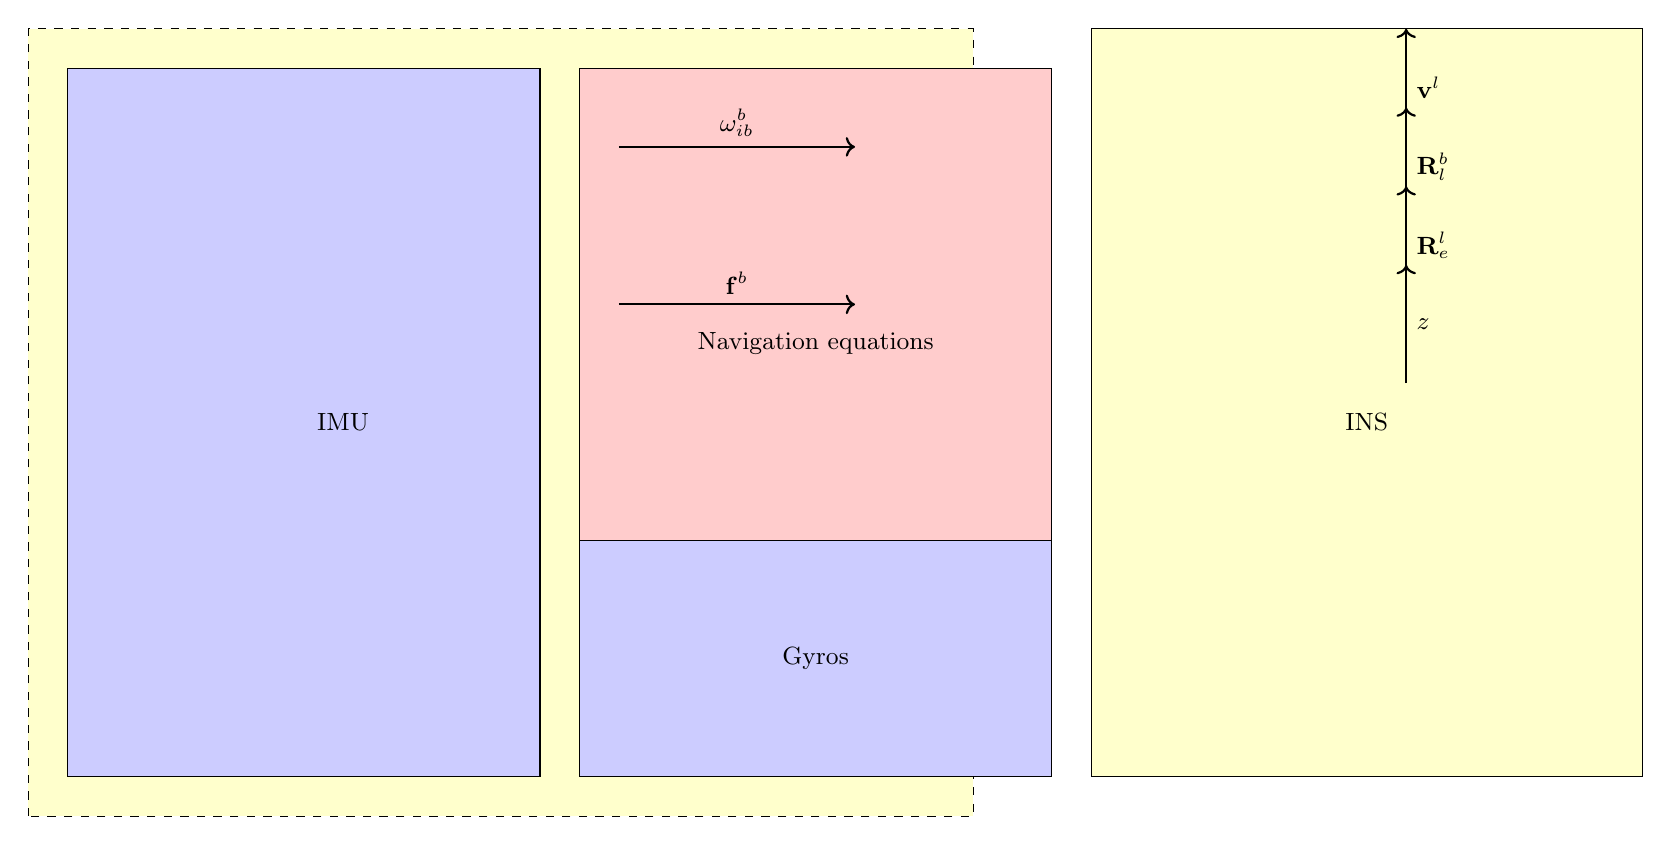
\begin{tikzpicture}[node distance=1cm, auto, font=\small]

% Define colors
\definecolor{lightyellow}{RGB}{255, 255, 204}
\definecolor{lightblue}{RGB}{204, 204, 255}
\definecolor{lightpink}{RGB}{255, 204, 204}

% Draw the main rectangle
\draw[fill=lightyellow, dashed] (0,0) rectangle (12,10);

% Draw the IMU section
\draw[fill=lightblue] (0.5,0.5) rectangle (6.5,9.5);
\node at (4,5) {IMU};

% Draw the gyros and accelerometers sections
\draw[fill=lightblue] (7,0.5) rectangle (13,3.5);
\node at (10,2) {Gyros};
\draw[fill=lightblue] (7,4.5) rectangle (13,7.5);
\node at (10,6) {Accelerometers};

% Draw the navigation equations section
\draw[fill=lightpink] (7,3.5) rectangle (13,9.5);
\node at (10,6) {Navigation equations};

% Draw the output section
\draw[fill=lightyellow] (13.5,0.5) rectangle (20.5,10);
\node at (17,5) {INS};

% Draw the arrows and labels
\draw[->, thick] (7.5,8.5) -- (10.5,8.5) node[midway, above] {$\omega_{ib}^b$};
\draw[->, thick] (7.5,6.5) -- (10.5,6.5) node[midway, above] {$\mathbf{f}^b$};
\draw[->, thick] (17.5,8.5) -- (17.5,10) node[midway, right] {$\mathbf{v}^l$};
\draw[->, thick] (17.5,7.5) -- (17.5,9) node[midway, right] {$\mathbf{R}_l^b$};
\draw[->, thick] (17.5,6.5) -- (17.5,8) node[midway, right] {$\mathbf{R}_e^l$};
\draw[->, thick] (17.5,5.5) -- (17.5,7) node[midway, right] {$z$};

\end{tikzpicture}

\end{document}